\section{Detailed design description}

%%%%%%%%%%%%%%%%%%%%%%%%%%%%%TODO genaue Beschreibung hier rein

% \begin{itemize}
% \item Description how the design will be implemented
% \item Event sequence digrams
% \item Internal structure
% 	\begin{itemize}
% 	\item Memory
% 	\item Logic blocks
% 	\item Parallel processes
% 	\item State machines
% 	\end{itemize}
% \end{itemize}

\subsection{Input}
\begin{figure}[!ht]
 \caption{State Machine des Input Moduls}
 \centering
 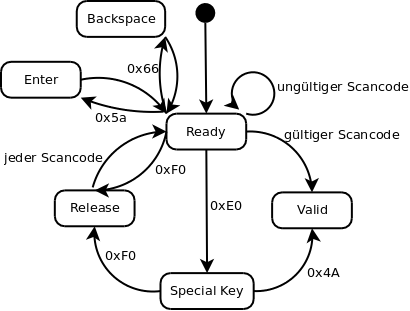
\includegraphics[scale=0.45]{pics/Input.png}
 \label{fig:Modules}
\end{figure}

Die Input Komponente empfängt die Scancodes vom PS2 Modul. Jedes Drücken der Tastatur löst ein bis drei Scancodes hintereinander aus.
Hier wird zwischen zwei Tasten unterschieden. 
\begin{itemize}
 \item Normale Tasten senden:\\
	\begin{itemize}
		\item einen Scancode beim Drücken
		\item zwei Scancodes, wobei der erste immer 0xF0 ist, beim Loslassen einer Taste und
		\item drei Scancodes 

	\end{itemize}
  \item Sondertasten, wie etwa die Enter Taste auf dem Nummernblock, senden:\\
  	Beim Drücken zwei und beim Loslassen drei Scancodes 
 \end{itemize}
Diese werden jeweils an die Input Komponente geschickt.
Die empfangenen Codes werden mit einem Lookup Table verglichen 
und weiter wie folgend verarbeitet.

Unterscheidung der Empfangenen Daten:
\begin{description}
 \item[0-9,+,-,*,/]
	\begin{itemize}
		\item Wandeln der Scancodes in ASCII chars 
		\item Speichern der Chars im RingBuffer
		\item Senden der Chars an den Output
	\end{itemize}
 \item[Enter] Senden an Parser und Output
 \item[Backspace] Senden an RingBuffer und Output
 \item[Space] Senden an RingBuffer und Output
 \item[Sonstige] Alle anderen Scancodes werden verworfen.
 \end{description}

Des Weiteren überwacht das Input Modul einen Button am development Board und sendet
daraufhin eine Anfrage an den SerialHandler

\subsection{Output}

\begin{figure}[!ht]
 \caption{State Machine des Output Moduls}
 \centering
 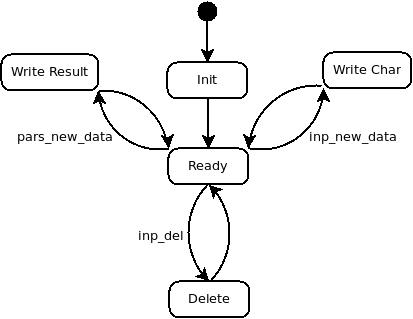
\includegraphics[scale=0.55]{pics/Output.png}
 \label{fig:output_module}
\end{figure}

Das Output Modul bekommt vom Input und vom Parser Nachrichten\\
\begin{description}
 \item[Vom Input] wird jeder ASCII Code oder die Backspace Taste an den Output geschickt. Diese werden
sofort an die VGA Komponente weiter gegeben und somit der Bildschirm aktualisiert. Hier wird auch überprüft ob
schon 70 Zeichen in der Rechnung sind und reagiert dann dementsprechend nur noch auf die Backspace Taste die das letzte Zeichen
löscht und den Cursor um eine Stelle nach hinten setzt.\\
 \item[Der Parser] schickt das Ergebnis an den Output. Durch das Empfangen des Ergebnisses weiß die Komponente
das die Rechnung vorbei ist. Es wird in die nächste Zeile gewechselt und danach ein '=' Zeichen und das Ergebnis
dahinter auf den Bildschirm geschrieben. Danach wird wieder in die nächste Zeile gewechselt und der Cursor dorthin
gesetzt. Somit kann die nächste Rechnung eingegeben werden.
 \end{description}
%TODO Signalnamen einsetzen
Über drei Signale kommuniziert der Output mit dem VGA Modul. Das signalname signalisiert uns das das VGA Modul 
frei ist und neue Befehle gesendet werden können. Wenn neue Befehle an den Output geschickt werden speichert das
Modul die Befehle zwischen und wartet bis die VGA Komponente frei ist. Mit signame1 wird er Befehl
gesendet und signame2 hilft beim Übernehmen des Signals.


\subsection{ALU}

\begin{figure}[!ht]
 \centering
 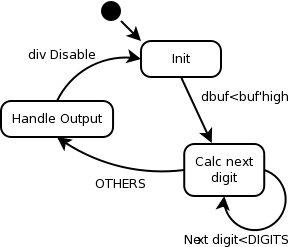
\includegraphics[scale=0.55]{pics/alu_div.png}
 \caption{State Machine des ALU Divisions Moduls}
 \label{fig:alu_div_module}
\end{figure}

\begin{figure}[!ht]
 \centering
 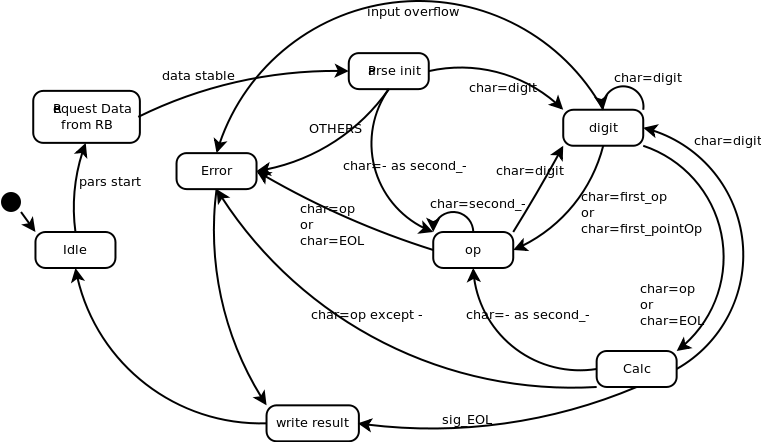
\includegraphics[scale=0.55]{pics/alu.png}
 \caption{State Machine der Alu}
 \label{fig:alu_module}
\end{figure}

Die ALU wird vom Parser zum Lösen simpler Berechnungen genützt. An die beiden Daten Eingänge \textit{calc\_data} werden die Operanden
und an \textit{calc\_operator} der Operator angelegt. Die Kodierung steht in folgender Tabelle:

\begin{center}
% use packages: array
\begin{tabular}[!ht]{|l|l|l|}
\hline calc\_operator (binär) & Rechenoperation & Rechnungsart\\ 
	\hline
	00 & Addieren & Strichrechnung\\ 
	01 & Subtrahieren & Strichrechnung\\ 
	10 & Multiplizieren & Punktrechnung\\ 
	11 & Dividieren & Punktrechnung\\
 \hline
\end{tabular}
\end{center}

Nachdem alle für die Berechnung benötigten Daten anliegen, wird mit dem Signal \textit{calc\_start} die Berechnung gestartet. \textit{calc\_finished}
sagt dem Parser, dass die Berechnung fertig ist. Sollte ein Fehler aufgetreten sein wird am \textit{calc\_error} ein Fehlercode gespeichert, der vom
Parser überprüft werden muss. Der Fehlercode steht in folgender Tabelle:

\begin{center}
% use packages: array
\begin{tabular}[!ht]{|l|l|}
\hline calc\_error (binär) & Fehler\\
	\hline
	00 & Fehlerfrei, Ergebnis gültig\\ 
	01 & Division durch Null\\ 
	10 & Overflow\\ 
	11 & reserviert\\
 \hline
\end{tabular}
\end{center}

Sollte kein Fehler vorgekommen sein, kann der Parser das Ergebnis auf \textit{calc\_data} ablesen. 

\subsection{Parser}

Der Parser löst die Gleichung, indem er die Rechnung in für ihn lösbare simple Rechnungen zerlegt.
Er wartet ihm durch den Input mit \textit{char\_EOL} gesagt wird die Rechnung zu lösen.\\
Der Parser holt sich dann vom Ringbuffer die momentane Zeile. Dann durchsucht er die Rechnung nach 
Punktrechnungen und löst diese der Reihe nach mit der ALU. Wenn keine mehr vorhanden sind wird
die Rechnung erneut auf Strichrechnungen durchsucht und der Reihe nach gelöst bis das Ergebnis 
fest steht.\\
Sollte die ALU in einem Schritt einen Overflow oder einen Divison durch Null Fehler bekommen wird 
die gesamte Rechnung gestoppt und an den Ringbuffer und dem Output eine Fehlermeldung geschickt.
Das selbe passiert wenn der Parser in einem Rechenschritt nicht die erwartete Syntax bekommt.\\

\subsection{Ringbuffer}

\begin{figure}[!ht]
 \caption{State Machine des Ringbuffer Moduls}
 \centering
 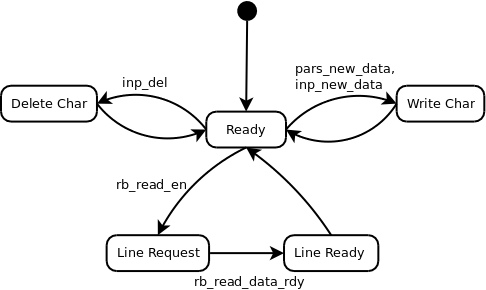
\includegraphics[scale=0.5]{pics/Ringbuffer.png}
 \label{fig:Modules}
\end{figure}

Der Ringbuffer ist grundsätzlich, wie der Name vermuten lässt, als Ringbuffer Struktur mit 50 Zeilen
zu je 81 Characters realisert. Es gibt einen Zeiger der auf die momentage Zeile zeigt. In dieser Zeile
steht die Rechnung die über die Tastatur eingegeben wurde und wird später vom Parser zur Berechnung
geholt. Wenn das Ergebnis vom Parser zu der Rechnung hinzugefügt wird, wird automatisch der interne Zeiger
auf die nächste Zeile verwiesen und der Inhalt der Zeile gelöscht, falls bereits mehr als 50 Rechnungen
eingegeben wurden.\\
Der Ringbuffer bekommt vom Input, über \textit{inp\_new\_data} und \textit{inp\_data}, und vom Parser, 
über \textit{pars\_new\_data} und \textit{pars\_data}, einzellne Characters zugeschickt.\\
Diese Characters werden, solange nicht mehr als 70 Zeichen in einer Zeile sind, in den Speicher geschrieben.
Vom Parser kriegt der Ringbuffer die einzellnen Zeichen des Ergebnisses. Das letzte Zeichen ist ein
Sonderzeichen worauf der Ringbuffer die momemtane Zeile beendet und den internen Zeiger auf die nächste
Zeile verweist und den Inhalt der Zeile löscht.\\
Wenn der Ringbuffer beschäftigt ist setzt er \textit{rb\_busy} auf High und signalisiert den anderen
Komponenten das keine neuen Zeichen gesendet werden dürfen.

\subsection{SerialHandler}

\begin{figure}[!ht]
 \caption{State Machine des SerialHandler Moduls}
 \centering
 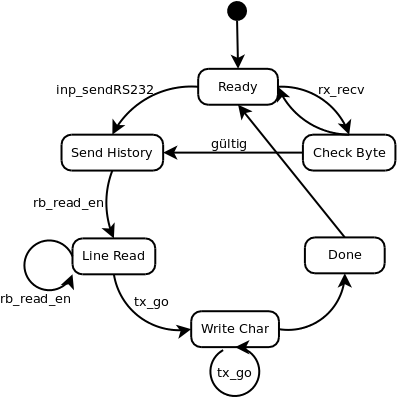
\includegraphics[scale=0.5]{pics/SerialHandler.png}
 \label{fig:Modules}
\end{figure}

Der SerialHandler dient als Schnittstelle zwischen dem Ringbuffer und dem RS232 Moduls. Wenn die ganze
History an den Computer geschickt werden soll kommt vom Input ein Signal, dass der Button am Entwicklerboard
gedrückt wurde. Außerdem kann dies durch das Senden eines Bytes auf dem RS232 Interface ebenfalls angefordert
werden.\\
Sobald dieser Request kommt wird vom Ringbuffer Zeile für Zeile eingelesen und danach jedes Zeichen
über das RS232 Modul an den PC geschickt.

\subsection{RS232}

\begin{figure}[!ht]
 \caption{State Machine des RS232 Moduls}
 \centering
 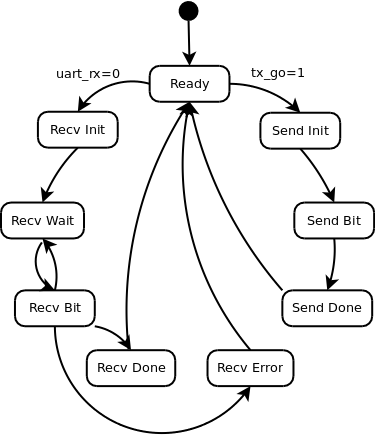
\includegraphics[scale=0.5]{pics/RS232.png}
 \label{fig:Modules}
\end{figure}

Das RS232 Modul wurde möglichst einfach gehalten. Es wartet bis es über das Signal 
\textit{tx\_go} vom SerialHandler der Befehl kommt neue Daten zu senden. Die Daten
werden über \textit{tx\_data} gelesen und über den Bus gesendet. Außerdem
hört die Komponente auf der Leitung ob Daten empfangen werden und signalisiert diese 
mit dem \textit{rc\_recv} Signal. Die vom RS232 Interface empfangenen Daten können 
dann über \textit{rx\_data} gelesen werden.\\
Gesendet und empfangen wird mit 8 Datenbits, einem Stopbit und keinem Paritätsbit, bei einer
Baudrate von 115`200.
%Senden: TX->LOW alle 8.68us nächstes Bit, dann 1 zum Stoppen
